\documentclass{ieeeaccess}
\usepackage{cite}
\usepackage{amsmath,amssymb,amsfonts}
\usepackage{algorithmic}
\usepackage{graphicx}
\usepackage{textcomp}
\def\BibTeX{{\rm B\kern-.05em{\sc i\kern-.025em b}\kern-.08em
    T\kern-.1667em\lower.7ex\hbox{E}\kern-.125emX}}
\begin{document}
\history{Date of publication xxxx 00, 0000, date of current version xxxx 00, 0000.}
\doi{10.1109/ACCESS.2023.0322000}

\title{Recurrent Neural Network based electricity theft detection}
\author{\uppercase{First A. Author}\authorrefmark{1}, \IEEEmembership{Fellow, IEEE},
\uppercase{Second B. Author}\authorrefmark{2}, and Third C. Author,
Jr.\authorrefmark{3},
\IEEEmembership{Member, IEEE}}

\address[1]{National Institute of Standards and
Technology, Boulder, CO 80305 USA (e-mail: author@boulder.nist.gov)}
\address[2]{Department of Physics, Colorado State University, Fort Collins,
CO 80523 USA (e-mail: author@lamar.colostate.edu)}
\address[3]{Electrical Engineering Department, University of Colorado, Boulder, CO
80309 USA}
\tfootnote{This paragraph of the first footnote will contain support
information, including sponsor and financial support acknowledgment. For
example, ``This work was supported in part by the U.S. Department of
Commerce under Grant BS123456.''}

\markboth
{Author \headeretal: Preparation of Papers for IEEE TRANSACTIONS and JOURNALS}
{Author \headeretal: Preparation of Papers for IEEE TRANSACTIONS and JOURNALS}

\corresp{Corresponding author: First A. Author (e-mail: author@ boulder.nist.gov).}


\begin{abstract}
Electricity is an essential part of modern life, powering everything from homes and businesses
to hospitals and schools and its theft is a widespread problem that affects many countries around the world. It
is estimated that electricity theft costs utility companies billions of dollars each year, while also endangering
the safety of both consumers and utility workers. Electricity theft can take many forms, from tampering with
meters to bypassing them altogether. Some individuals may also connect directly to power lines, which can
be incredibly dangerous and potentially deadly. The reasons for electricity theft vary, but often involve a
desire to avoid paying for electricity or to generate income through the sale of stolen electricity. Theft also
poses a significant safety risk to both consumers and utility workers. Tampering with electrical systems can
lead to fires and electrocution, which can cause serious injury or death. Preventing electricity theft requires
a multi-faceted approach. One key strategy is to improve metering systems, which can detect and prevent
unauthorized access to electricity. Additionally, governments can increase penalties for those caught stealing
electricity, which can act as a deterrent to potential thieves, etc. This paper aims a different method for theft
detection which uses comprehensive features in time and frequency domains in a recurrent neural network-
based classification approach usig LSTM.
\end{abstract}

\begin{keywords}
Recurrent neural network, machine learning, electricity theft, lstm
\end{keywords}

\titlepgskip=-21pt

\maketitle

\section{Introduction}
\label{sec:introduction}
\PARstart{E}{lectricity} is a crucial necessity in today's modern society. It fuels industries, transportation, residences, and workplaces. However, despite its significance, many regions of the world continue to have problems with a lack of electricity, high costs, and theft.
Particularly in many nations worldwide, electricity theft is a serious issue. Electricity theft happens when people or organizations improperly access the electrical system, evading the meter and failing to pay for the electricity they consume. This practice contributes significantly to the insufficient supply of power and costs governments and electricity suppliers billions of dollars annually.


There are several causes of electricity theft. In some circumstances, it is because people are too poor to purchase the electricity they require. In other instances, it is the result of corruption, where some people or companies engage in criminal activity to profit. Sometimes it's because there isn't enough enforcement by the authorities, which makes it simpler for people to steal electricity without worrying about getting caught.
Governments and electrical companies must adopt a multifaceted strategy to address electricity theft. This entails enhancing access to electricity for people who cannot afford it, toughening up on electricity theft, and putting detection and prevention mechanisms in place. Innovative grid technologies, which employ digital monitoring systems to quickly identify and pinpoint electricity theft, have been adopted in several nations.


In developing nations, the problem of insufficient electrical supply is particularly pronounced. Many people in these areas don't have access to power, and those who do frequently experience blackouts because of inadequate infrastructure and supply. Access to vital services like healthcare, education, and communication is impacted by energy availability, which inhibits economic growth and development.
There are many causes of insufficient electrical supply. In certain circumstances, especially in rural areas, it results from a lack of infrastructure investment. Other times, it's because of inefficient resource use, which causes power shortages during demand times. In certain instances, it's because of political unrest, which disrupts the supply chain.


Governments and electrical suppliers must invest in infrastructure, especially in rural regions, to address the problem of a lack of electricity supply. Additionally, they must develop renewable energy sources like wind and solar, which are more resilient and sustainable to supply chain shocks. They also need to promote energy efficiency and decrease waste because doing so will assist to balance supply and demand.
A further big issue that many individuals deal with is the price of electricity. Electricity costs are excessive in several nations, making them unaffordable for many people and enterprises. Electricity subsidies in other nations result in underinvestment in infrastructure and wasteful resource utilization.


In conclusion, electricity is an essential resource for contemporary society, yet it is still a problem in many regions of the world due to low availability, excessive prices, and theft. Governments and electrical suppliers must adopt a multifaceted strategy to tackle these issues, one that includes spending money on infrastructure, creating renewable energy sources, increasing energy efficiency, and putting in place tools to stop and detect theft. Then and only then can we guarantee that everyone has access to safe, dependable electricity.

In this paper, we provide an efficient electricity theft detection method based on carefully extracted and selected features in Recurrent Neural Network (RNN)-based classification approach. We demonstrate that employing frequency-domain features as opposed to using time-domain features alone enhances classification performance. We use a realistic electricity consumption dataset released by the State Grid Corporation of China (SGCC) accessible at [1]. The dataset comprises electricity usage statistics recorded from January 2014 to October 2016. The main contributions are as follows:
\begin{itemize}

\item We propose a unique RNN classification-based electricity theft detection method using extensive time-domain features. We further propose using frequency-domain features to enhance performance.

\item We optimize the hyperparameters of the model for overall improved performance using a random search that can be employed to obtain good outcomes with optimal model training speed. 

\end{itemize}

\section{Related Work}
Use either SI (MKS) or CGS as primary units. (SI units are strongly
encouraged.) English units may be used as secondary units (in parentheses).
This applies to papers in data storage. For example, write ``15
Gb/cm$^{2}$ (100 Gb/in$^{2})$.'' An exception is when
English units are used as identifiers in trade, such as ``3$^{1\!/\!2}$-in
disk drive.'' Avoid combining SI and CGS units, such as current in amperes
and magnetic field in oersteds. This often leads to confusion because
equations do not balance dimensionally. If you must use mixed units, clearly
state the units for each quantity in an equation.

The SI unit for magnetic field strength $H$ is A/m. However, if you wish to use
units of T, either refer to magnetic flux density $B$ or magnetic field
strength symbolized as $\mu _{0}H$. Use the center dot to separate
compound units, e.g., ``A$\cdot $m$^{2}$.''

\section{PRELIMINARIES}
Recurrent Neural Network is referred to as RNN. It is a kind of neural network with memory that works best with sequential data. Google Voice Search and Apple's Siri both employ RNN. Let’s explain the basic basics of RNN and understand Forward Propagation and Backward Propagation before diving deeper.

\subsection{Forward and Backward Propagation}
\subsubsection{Forward Propagation}
The simplest kind of neural network is this one. Data flows only in forward direction from input layer to hidden layers to the output layer. It could have one or more secret layers. Each node has complete connectivity.To obtain the output of the model, assess its accuracy, and determine the error, we use forward propagation.

\subsubsection{Backward Propagation}
Training neural networks is done using the back propagation approach. Deep neural networks may be used if there are numerous hidden layers. We compute the error when forward propagation is finished. The network then receives a back-propagation of this error to update the weights. We move backward through the neural network to get the partial derivatives of the error (loss function) with respect to the weights. To determine step size, this partial derivative is now multiplied by the learning rate. To determine new weights, the step size is applied to the initial weights. A neural network learns in this manner while being trained.

\subsection{What is RNN?}
A feed-forward neural network with internal memory is referred to as a recurrent neural network. The result of the current input depends on the previous computation, making RNNs recurrent in nature because they carry out the same function for every data input. The output is created, copied, and then delivered back into the recurrent network. It takes into account both the current input and the output that it has learned from the prior input when making a decision.

RNNs can process input sequences using their internal state (memory), in contrast to feed-forward neural networks. They can therefore be used for tasks like connected, unsegmented handwriting recognition or speech recognition. All of the inputs in other neural networks operate independently of one another. However, with RNN, every input is connected to every other input.

\Figure[t!](topskip=0pt, botskip=0pt, midskip=0pt)[width=0.98\linewidth]{fig1.png}
{ \textbf{Recurrent neural network.}\label{fig1}}

\subsubsection{Best suited for sequential data}
Sequential data is where RNN shines the most. Any input or output length is supported. RNN processes arbitrary input sequences using its internal memory. RNNs are therefore the most effective in predicting the following words in a string of words. Like a human brain, particularly in dialogues, more weight is given to recency of information to predict sentences. A RNN that has been taught to translate text might discover that the word "dog" should be translated differently if the word "hot" comes before it.

\subsubsection{RNN has internal memory}
RNN is capable of having memory. Data from the past is retained. While making a decision, it takes into consideration the current input and also what it has learned from the inputs it received previously. A feedback loop is created when the output from the previous step is used as the input for the current step. As a result, it uses the set of current input and the past state to determine its current state. In this way, the information cycles through a loop. In a nutshell, we can say that RNN has two inputs, the present and the recent past. This is significant because the sequence of data carries crucial information about what is coming next, which is why an RNN can achieve things other algorithms can’t.

\subsection{How does RNN work?}
Recurrent neural networks (RNNs) are a subclass of neural networks that are capable of processing sequences of inputs, such as time-series data or text written in English language, by maintaining a state that stores details about the previous inputs. In order to create an output, this state and the current input are both sent across the network. An RNN can learn to predict the future or produce output sequences based on the context of its prior inputs in this fashion.

RNNs can be visualised as a series of repeating modules, where each module accepts the input and output from the module before it as input. The recurrent link, which permits information to be transmitted from one time step to the next, is the essential component that allows RNNs to capture sequential data.

The simple recurrent unit, or SRU, is the most fundamental type of RNN module and is defined as follows:
\[ h_t=f(Wx_t+Uh_{t-1}+b )\]

\Figure[t!](topskip=13pt, botskip=0pt, midskip=0pt)[width=0.98\linewidth]{Rnn-architecture.jpg}
{ \textbf{Architecture of Recurrent neural network.}\label{fig2}}

where \(h_t\) is the hidden state at time step \(t\), \({x_t}\) is the input at time step \(t\), \(W\) and \(U\) are weight matrices, \(b\) is the bias vector, and \(f\) is the activation function, such as the sigmoid function or the hyperbolic tangent function.

This equation describes how the hidden state \(h_t\) is computed as a function of the input \(x_t\) and the previous hidden state \(h_{t-1}\), using a linear transformation of the inputs and the previous hidden state, followed by a non-linear activation function.

In order to train an RNN, we need to compute the gradient of the loss function with respect to the parameters of the network, and update the parameters using an optimization algorithm such as stochastic gradient descent. The challenge in training RNNs is that the gradient can become very small or very large over time, due to the repeated multiplication of the weight matrices \(W\) and \(U\). This can lead to the vanishing or exploding gradient problem, which makes it difficult to learn long-term dependencies in the input sequence.

One solution to this problem is to use a variant of the SRU called the Long Short-Term Memory (LSTM) unit, which uses gates to control the flow of information through the network. Another solution is the Gated Recurrent Unit (GRU), which uses a simpler gating mechanism than the LSTM.

Overall, RNNs are a powerful tool for processing sequential data, but require careful tuning and regularization to avoid the vanishing or exploding gradient problem.


\section{RNN-BASED ELECTRICITY THEFT DETECTION METHOD}
The electricity theft detection method outlined in this section consists of the following three steps: Data Analysis and Pre- processing, Feature Extraction, and Classification
\label{sec:guidelines}

\subsection{DATA ANALYSIS AND PRE-PROCESSING}
We used a realistic electricity consumption dataset released by SGCC, which can be accessed at [1]. The dataset consists of daily electricity consumption data taken from January 2014 to October 2016, summarized in Table 1. 

The sampling rate of the data is uniform for every customer, it is one measurement per day, which corresponds to the total power consumption for that day. The used dataset consists of 42372 observations, of which 3615 observations are electricity consumption data of unfaithful customers and the remaining observations are electricity consumption data of faithful customers.

\subsubsection{Color/Grayscale figures}
{Figures that are meant to appear in color, or shades of black/gray. Such
figures may include photographs, illustrations, multicolor graphs, and
flowcharts. For multicolor graphs, please avoid any gray backgrounds or shading, as well as screenshots, instead export the graph from the program used to collect the data.}

\subsubsection{Line Art figures}
{Figures that are composed of only black lines and shapes. These figures
should have no shades or half-tones of gray, only black and white.}

\subsubsection{Author photos}
{Author photographs should be included with the author biographies located at the end of the article underneath References. }



\subsection{Multipart figures}
Figures compiled of more than one sub-figure presented side-by-side, or
stacked. If a multipart figure is made up of multiple figure
types (one part is lineart, and another is grayscale or color) the figure
should meet the stricter guidelines.

\subsection{File Formats For Graphics}\label{formats}
Format and save your graphics using a suitable graphics processing program
that will allow you to create the images as PostScript (.PS), Encapsulated
PostScript (.EPS), Tagged Image File Format (.TIFF), Portable Document
Format (.PDF), Portable Network Graphics (.PNG), or Metapost (.MPS), sizes them, and adjusts
the resolution settings. When
submitting your final paper, your graphics should all be submitted
individually in one of these formats along with the manuscript.

\subsection{Sizing of Graphics}
Most charts, graphs, and tables are one column wide (3.5 inches/88
millimeters/21 picas) or page wide (7.16 inches/181 millimeters/43
picas). The maximum depth a graphic can be is 8.5 inches (216 millimeters/54
picas). When choosing the depth of a graphic, please allow space for a
caption. Figures can be sized between column and page widths if the author
chooses, however it is recommended that figures are not sized less than
column width unless when necessary.

There is currently one publication with column measurements that do not
coincide with those listed above. Proceedings of the IEEE has a column
measurement of 3.25 inches (82.5 millimeters/19.5 picas).

The final printed size of author photographs is exactly
1 inch wide by 1.25 inches tall (25.4 millimeters$\,\times\,$31.75 millimeters/6
picas$\,\times\,$7.5 picas). Author photos printed in editorials measure 1.59 inches
wide by 2 inches tall (40 millimeters$\,\times\,$50 millimeters/9.5 picas$\,\times\,$12
picas).

\subsection{Resolution }
The proper resolution of your figures will depend on the type of figure it
is as defined in the ``Types of Figures'' section. Author photographs,
color, and grayscale figures should be at least 300dpi. Line art, including
tables should be a minimum of 600dpi.

\subsection{Vector Art}
In order to preserve the figures' integrity across multiple computer
platforms, we accept files in the following formats: .EPS/.PDF/.PS. All
fonts must be embedded or text converted to outlines in order to achieve the
best-quality results.

\subsection{Color Space}
The term color space refers to the entire sum of colors that can be
represented within the said medium. For our purposes, the three main color
spaces are Grayscale, RGB (red/green/blue) and CMYK
(cyan/magenta/yellow/black). RGB is generally used with on-screen graphics,
whereas CMYK is used for printing purposes.

All color figures should be generated in RGB or CMYK color space. Grayscale
images should be submitted in Grayscale color space. Line art may be
provided in grayscale OR bitmap colorspace. Note that ``bitmap colorspace''
and ``bitmap file format'' are not the same thing. When bitmap color space
is selected, .TIF/.TIFF/.PNG are the recommended file formats.

\subsection{Accepted Fonts Within Figures}
When preparing your graphics IEEE suggests that you use of one of the
following Open Type fonts: Times New Roman, Helvetica, Arial, Cambria, and
Symbol. If you are supplying EPS, PS, or PDF files all fonts must be
embedded. Some fonts may only be native to your operating system; without
the fonts embedded, parts of the graphic may be distorted or missing.

A safe option when finalizing your figures is to strip out the fonts before
you save the files, creating ``outline'' type. This converts fonts to
artwork what will appear uniformly on any screen.

\subsection{Using Labels Within Figures}

\subsubsection{Figure Axis labels }
Figure axis labels are often a source of confusion. Use words rather than
symbols. As an example, write the quantity ``Magnetization,'' or
``Magnetization M,'' not just ``M.'' Put units in parentheses. Do not label
axes only with units. As in Fig. 1, for example, write ``Magnetization
(A/m)'' or ``Magnetization (A$\cdot$m$^{-1}$),'' not just ``A/m.'' Do not label axes with a ratio of quantities and
units. For example, write ``Temperature (K),'' not ``Temperature/K.''

Multipliers can be especially confusing. Write ``Magnetization (kA/m)'' or
``Magnetization (10$^{3}$ A/m).'' Do not write ``Magnetization
(A/m)$\,\times\,$1000'' because the reader would not know whether the top
axis label in Fig. 1 meant 16000 A/m or 0.016 A/m. Figure labels should be
legible, approximately 8 to 10 point type.

\subsubsection{Subfigure Labels in Multipart Figures and Tables}
Multipart figures should be combined and labeled before final submission.
Labels should appear centered below each subfigure in 8 point Times New
Roman font in the format of (a) (b) (c).

\subsection{File Naming}
Figures (line artwork or photographs) should be named starting with the
first 5 letters of the author's last name. The next characters in the
filename should be the number that represents the sequential
location of this image in your article. For example, in author
``Anderson's'' paper, the first three figures would be named ander1.tif,
ander2.tif, and ander3.ps.

Tables should contain only the body of the table (not the caption) and
should be named similarly to figures, except that `.t' is inserted
in-between the author's name and the table number. For example, author
Anderson's first three tables would be named ander.t1.tif, ander.t2.ps,
ander.t3.eps.

Author photographs should be named using the first five characters of the
pictured author's last name. For example, four author photographs for a
paper may be named: oppen.ps, moshc.tif, chen.eps, and duran.pdf.

If two authors or more have the same last name, their first initial(s) can
be substituted for the fifth, fourth, third$\ldots$ letters of their surname
until the degree where there is differentiation. For example, two authors
Michael and Monica Oppenheimer's photos would be named oppmi.tif, and
oppmo.eps.

\subsection{Referencing a Figure or Table Within Your Paper}
When referencing your figures and tables within your paper, use the
abbreviation ``Fig.'' even at the beginning of a sentence. Figures should be numbered with Arabic Numerals.
Do not abbreviate ``Table.'' Tables should be numbered with Roman Numerals.

\subsection{Submitting Your Graphics}
Because IEEE will do the final formatting of your paper,
you do not need to position figures and tables at the top and bottom of each
column. In fact, all figures, figure captions, and tables can be placed at
the end of your paper. In addition to, or even in lieu of submitting figures
within your final manuscript, figures should be submitted individually,
separate from the manuscript in one of the file formats listed above in
Section \ref{formats}. Place figure captions below the figures; place table titles
above the tables. Please do not include captions as part of the figures, or
put them in ``text boxes'' linked to the figures. Also, do not place borders
around the outside of your figures.

\subsection{Color Processing/Printing in IEEE Journals}
All IEEE Transactions, Journals, and Letters allow an author to publish
color figures on IEEE {\it Xplore}$\circledR$\ at no charge, and automatically
convert them to grayscale for print versions. In most journals, figures and
tables may alternatively be printed in color if an author chooses to do so.
Please note that this service comes at an extra expense to the author. If
you intend to have print color graphics, include a note with your final
paper indicating which figures or tables you would like to be handled that
way, and stating that you are willing to pay the additional fee.

\section{RESULTS AND DISCUSSION}
The word ``data'' is plural, not singular. The subscript for the
permeability of vacuum $\mu _{0}$ is zero, not a lowercase letter
``o.'' The term for residual magnetization is ``remanence''; the adjective
is ``remanent''; do not write ``remnance'' or ``remnant.'' Use the word
``micrometer'' instead of ``micron.'' A graph within a graph is an
``inset,'' not an ``insert.'' The word ``alternatively'' is preferred to the
word ``alternately'' (unless you really mean something that alternates). Use
the word ``whereas'' instead of ``while'' (unless you are referring to
simultaneous events). Do not use the word ``essentially'' to mean
``approximately'' or ``effectively.'' Do not use the word ``issue'' as a
euphemism for ``problem.'' When compositions are not specified, separate
chemical symbols by en-dashes; for example, ``NiMn'' indicates the
intermetallic compound Ni$_{0.5}$Mn$_{0.5}$ whereas
``Ni--Mn'' indicates an alloy of some composition
Ni$_{x}$Mn$_{1-x}$.

Be aware of the different meanings of the homophones ``affect'' (usually a
verb) and ``effect'' (usually a noun), ``complement'' and ``compliment,''
``discreet'' and ``discrete,'' ``principal'' (e.g., ``principal
investigator'') and ``principle'' (e.g., ``principle of measurement''). Do
not confuse ``imply'' and ``infer.''

Prefixes such as ``non,'' ``sub,'' ``micro,'' ``multi,'' and ``ultra'' are
not independent words; they should be joined to the words they modify,
usually without a hyphen. There is no period after the ``et'' in the Latin
abbreviation ``\emph{et al.}'' (it is also italicized). The abbreviation ``i.e.,'' means
``that is,'' and the abbreviation ``e.g.,'' means ``for example'' (these
abbreviations are not italicized).

A general IEEE styleguide is available at \break
\underline{http://www.ieee.org/authortools}.

\section{Conclusion}
Although a conclusion may review the  main points of the paper, do not replicate the abstract as the conclusion. A
conclusion might elaborate on the importance of the work or suggest
applications and extensions.

If you have multiple appendices, use the $\backslash$appendices command below. If you have only one appendix, use
$\backslash$appendix[Appendix Title]


\begin{thebibliography}{00}

\bibitem{b1} Z. Zheng, Y. Yang, X. Niu, H.-N. Dai, and Y. Zhou. (Sep. 30, 2021). Electricity Theft Detection, [Online]. Available: https://github.com/henryRDlab/ ElectricityTheftDetection

\bibitem{b2} W.-K. Chen, \emph{Linear Networks and Systems.} Belmont, CA, USA: Wadsworth, 1993, pp. 123--135.

\bibitem{b3} J. U. Duncombe, ``Infrared navigation---Part I: An assessment of feasibility,'' \emph{IEEE Trans. Electron Devices}, vol. ED-11, no. 1, pp. 34--39, Jan. 1959, 10.1109/TED.2016.2628402.

\bibitem{b4} E. P. Wigner, ``Theory of traveling-wave optical laser,'' \emph{Phys. Rev}., vol. 134, pp. A635--A646, Dec. 1965.

\bibitem{b5} E. H. Miller, ``A note on reflector arrays,'' \emph{IEEE Trans. Antennas Propagat}., to be published.

\bibitem{b6} E. E. Reber, R. L. Michell, and C. J. Carter, ``Oxygen absorption in the earth's atmosphere,'' Aerospace Corp., Los Angeles, CA, USA, Tech. Rep. TR-0200 (4230-46)-3, Nov. 1988.

\bibitem{b7} J. H. Davis and J. R. Cogdell, ``Calibration program for the 16-foot antenna,'' Elect. Eng. Res. Lab., Univ. Texas, Austin, TX, USA, Tech. Memo. NGL-006-69-3, Nov. 15, 1987.

\bibitem{b8} \emph{Transmission Systems for Communications}, 3\textsuperscript{rd} ed., Western Electric Co., Winston-Salem, NC, USA, 1985, pp. 44--60.

\bibitem{b9} \emph{Motorola Semiconductor Data Manual}, Motorola Semiconductor Products Inc., Phoenix, AZ, USA, 1989.

\bibitem{b10} G. O. Young, ``Synthetic structure of industrial
plastics,'' in Plastics, vol. 3, Polymers of Hexadromicon, J. Peters,
Ed., 2\textsuperscript{nd} ed. New York, NY, USA: McGraw-Hill, 1964, pp. 15-64.
[Online]. Available:
\underline{http://www.bookref.com}.

\bibitem{b11} \emph{The Founders' Constitution}, Philip B. Kurland
and Ralph Lerner, eds., Chicago, IL, USA: Univ. Chicago Press, 1987.
[Online]. Available: \underline{http://press-pubs.uchicago.edu/founders/}

\bibitem{b12} The Terahertz Wave eBook. ZOmega Terahertz Corp., 2014.
[Online]. Available:
\underline{http://dl.z-thz.com/eBook/zomegaebookpdf\_1206\_sr.pdf}. Accessed on: May 19, 2014.

\bibitem{b13} Philip B. Kurland and Ralph Lerner, eds., \emph{The
Founders' Constitution.} Chicago, IL, USA: Univ. of Chicago Press,
1987, Accessed on: Feb. 28, 2010, [Online] Available:
\underline{http://press-pubs.uchicago.edu/founders/}

\bibitem{b14} J. S. Turner, ``New directions in communications,'' \emph{IEEE J. Sel. Areas Commun}., vol. 13, no. 1, pp. 11-23, Jan. 1995.

\bibitem{b15} W. P. Risk, G. S. Kino, and H. J. Shaw, ``Fiber-optic frequency shifter using a surface acoustic wave incident at an oblique angle,'' \emph{Opt. Lett.}, vol. 11, no. 2, pp. 115--117, Feb. 1986.

\bibitem{b16} P. Kopyt \emph{et al., ``}Electric properties of graphene-based conductive layers from DC up to terahertz range,'' \emph{IEEE THz Sci. Technol.,} to be published. DOI: 10.1109/TTHZ.2016.2544142.

\bibitem{b17} PROCESS Corporation, Boston, MA, USA. Intranets:
Internet technologies deployed behind the firewall for corporate
productivity. Presented at INET96 Annual Meeting. [Online].
Available: \underline{http://home.process.com/Intranets/wp2.htp}

\bibitem{b18} R. J. Hijmans and J. van Etten, ``Raster: Geographic analysis and modeling with raster data,'' R Package Version 2.0-12, Jan. 12, 2012. [Online]. Available: \underline {http://CRAN.R-project.org/package=raster}

\bibitem{b19} Teralyzer. Lytera UG, Kirchhain, Germany [Online].
Available:
\underline{http://www.lytera.de/Terahertz\_THz\_Spectroscopy.php?id=home}, Accessed on: Jun. 5, 2014.

\bibitem{b20} U.S. House. 102\textsuperscript{nd} Congress, 1\textsuperscript{st} Session. (1991, Jan. 11). \emph{H. Con. Res. 1, Sense of the Congress on Approval of}  \emph{Military Action}. [Online]. Available: LEXIS Library: GENFED File: BILLS

\bibitem{b21} Musical toothbrush with mirror, by L.M.R. Brooks. (1992, May 19). Patent D 326 189 [Online]. Available: NEXIS Library: LEXPAT File: DES

\bibitem{b22} D. B. Payne and J. R. Stern, ``Wavelength-switched pas- sively coupled single-mode optical network,'' in \emph{Proc. IOOC-ECOC,} Boston, MA, USA, 1985, pp. 585--590.

\bibitem{b23} D. Ebehard and E. Voges, ``Digital single sideband detection for interferometric sensors,'' presented at the \emph{2\textsuperscript{nd} Int. Conf. Optical Fiber Sensors,} Stuttgart, Germany, Jan. 2-5, 1984.

\bibitem{b24} G. Brandli and M. Dick, ``Alternating current fed power supply,'' U.S. Patent 4 084 217, Nov. 4, 1978.

\bibitem{b25} J. O. Williams, ``Narrow-band analyzer,'' Ph.D. dissertation, Dept. Elect. Eng., Harvard Univ., Cambridge, MA, USA, 1993.

\bibitem{b26} N. Kawasaki, ``Parametric study of thermal and chemical nonequilibrium nozzle flow,'' M.S. thesis, Dept. Electron. Eng., Osaka Univ., Osaka, Japan, 1993.

\bibitem{b27} A. Harrison, private communication, May 1995.

\bibitem{b28} B. Smith, ``An approach to graphs of linear forms,'' unpublished.

\bibitem{b29} A. Brahms, ``Representation error for real numbers in binary computer arithmetic,'' IEEE Computer Group Repository, Paper R-67-85.

\bibitem{b30} IEEE Criteria for Class IE Electric Systems, IEEE Standard 308, 1969.

\bibitem{b31} Letter Symbols for Quantities, ANSI Standard Y10.5-1968.

\bibitem{b32} R. Fardel, M. Nagel, F. Nuesch, T. Lippert, and A. Wokaun, ``Fabrication of organic light emitting diode pixels by laser-assisted forward transfer,'' \emph{Appl. Phys. Lett.}, vol. 91, no. 6, Aug. 2007, Art. no. 061103.~

\bibitem{b33} J. Zhang and N. Tansu, ``Optical gain and laser characteristics of InGaN quantum wells on ternary InGaN substrates,'' \emph{IEEE Photon. J.}, vol. 5, no. 2, Apr. 2013, Art. no. 2600111

\bibitem{b34} S. Azodolmolky~\emph{et al.}, Experimental demonstration of an impairment aware network planning and operation tool for transparent/translucent optical networks,''~\emph{J. Lightw. Technol.}, vol. 29, no. 4, pp. 439--448, Sep. 2011.

\end{thebibliography}

\begin{IEEEbiography}[{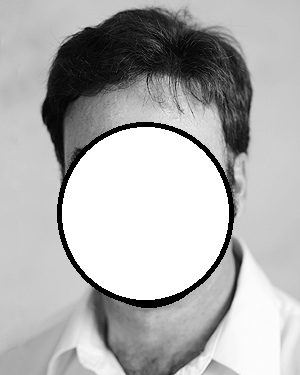
\includegraphics[width=1in,height=1.25in,clip,keepaspectratio]{author1.png}}]{First A. Author} received the B.S. and M.S. degrees in aerospace engineering from
the University of Virginia, Charlottesville, in 2001 and the Ph.D. degree in
mechanical engineering from Drexel University, Philadelphia, PA, in 2008.

From 2001 to 2004, he was a Research Assistant with the Princeton Plasma
Physics Laboratory. Since 2009, he has been an Assistant Professor with the
Mechanical Engineering Department, Texas A{\&}M University, College Station.
He is the author of three books, more than 150 articles, and more than 70
inventions. His research interests include high-pressure and high-density
nonthermal plasma discharge processes and applications, microscale plasma
discharges, discharges in liquids, spectroscopic diagnostics, plasma
propulsion, and innovation plasma applications. He is an Associate Editor of
the journal \emph{Earth, Moon, Planets}, and holds two patents.

Dr. Author was a recipient of the International Association of Geomagnetism
and Aeronomy Young Scientist Award for Excellence in 2008, and the IEEE
Electromagnetic Compatibility Society Best Symposium Paper Award in 2011.
\end{IEEEbiography}


\begin{IEEEbiography}[{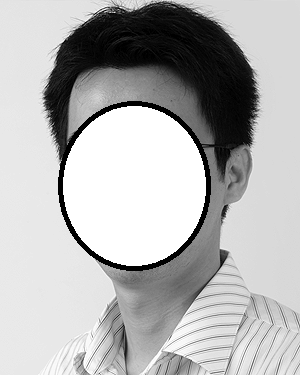
\includegraphics[width=1in,height=1.25in,clip,keepaspectratio]{author3.png}}]{Third C. Author, Jr.} (M'87) received the B.S. degree in mechanical
engineering from National Chung Cheng University, Chiayi, Taiwan, in 2004
and the M.S. degree in mechanical engineering from National Tsing Hua
University, Hsinchu, Taiwan, in 2006. He is currently pursuing the Ph.D.
degree in mechanical engineering at Texas A{\&}M University, College
Station, TX, USA.

From 2008 to 2009, he was a Research Assistant with the Institute of
Physics, Academia Sinica, Tapei, Taiwan. His research interest includes the
development of surface processing and biological/medical treatment
techniques using nonthermal atmospheric pressure plasmas, fundamental study
of plasma sources, and fabrication of micro- or nanostructured surfaces.

Mr. Author's awards and honors include the Frew Fellowship (Australian
Academy of Science), the I. I. Rabi Prize (APS), the European Frequency and
Time Forum Award, the Carl Zeiss Research Award, the William F. Meggers
Award and the Adolph Lomb Medal (OSA).
\end{IEEEbiography}

\begin{IEEEbiography}[{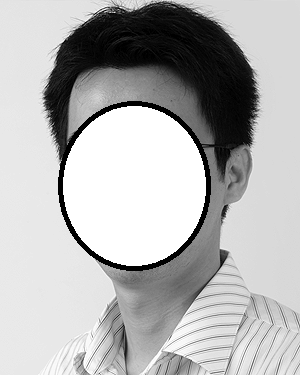
\includegraphics[width=1in,height=1.25in,clip,keepaspectratio]{author3.png}}]{Third C. Author, Jr.} (M'87) received the B.S. degree in mechanical
engineering from National Chung Cheng University, Chiayi, Taiwan, in 2004
and the M.S. degree in mechanical engineering from National Tsing Hua
University, Hsinchu, Taiwan, in 2006. He is currently pursuing the Ph.D.
degree in mechanical engineering at Texas A{\&}M University, College
Station, TX, USA.

From 2008 to 2009, he was a Research Assistant with the Institute of
Physics, Academia Sinica, Tapei, Taiwan. His research interest includes the
development of surface processing and biological/medical treatment
techniques using nonthermal atmospheric pressure plasmas, fundamental study
of plasma sources, and fabrication of micro- or nanostructured surfaces.

Mr. Author's awards and honors include the Frew Fellowship (Australian
Academy of Science), the I. I. Rabi Prize (APS), the European Frequency and
Time Forum Award, the Carl Zeiss Research Award, the William F. Meggers
Award and the Adolph Lomb Medal (OSA).
\end{IEEEbiography}

\begin{IEEEbiography}[{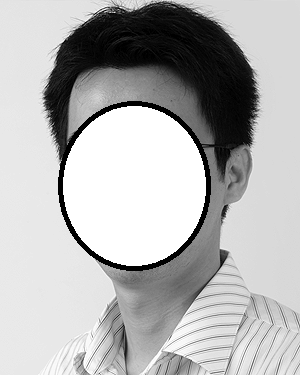
\includegraphics[width=1in,height=1.25in,clip,keepaspectratio]{author3.png}}]{Third C. Author, Jr.} (M'87) received the B.S. degree in mechanical
engineering from National Chung Cheng University, Chiayi, Taiwan, in 2004
and the M.S. degree in mechanical engineering from National Tsing Hua
University, Hsinchu, Taiwan, in 2006. He is currently pursuing the Ph.D.
degree in mechanical engineering at Texas A{\&}M University, College
Station, TX, USA.

From 2008 to 2009, he was a Research Assistant with the Institute of
Physics, Academia Sinica, Tapei, Taiwan. His research interest includes the
development of surface processing and biological/medical treatment
techniques using nonthermal atmospheric pressure plasmas, fundamental study
of plasma sources, and fabrication of micro- or nanostructured surfaces.

Mr. Author's awards and honors include the Frew Fellowship (Australian
Academy of Science), the I. I. Rabi Prize (APS), the European Frequency and
Time Forum Award, the Carl Zeiss Research Award, the William F. Meggers
Award and the Adolph Lomb Medal (OSA).
\end{IEEEbiography}


\EOD

\end{document}
